\documentclass[jou]{apa6}
\usepackage[utf8]{inputenc}
\usepackage[spanish]{babel}

\usepackage{csquotes}
\usepackage[style=apa,sortcites=true,sorting=nyt,backend=biber]{biblatex}

\usepackage{listings}

\usepackage[section]{placeins}

\DeclareLanguageMapping{spanish}{spanish-apa}
\addbibresource{bibliography.bib}

\title{HPC - LAb2: OpenMP}

\author{Rubén Cavieres Carvajal}
\affiliation{Universidad de Santiago de Chile}

\leftheader{DIINF-USACH}

\abstract{Se presenta un resumen del desarrollo del laboratorio 2 de la asignatura High Performance Computing dictado por el profesor Dr. Fernando Rannou, exponiendo resultados de las pruebas de rendimiento computacional sobre la aplicación paralelizada.}

\keywords{HPC, OpenMP, Parallel, Schroedinger}

\begin{document}
\maketitle
El trabajo comienza con la creación de un algoritmo secuencial que simula el comportamiento de una onda bajo la ley de Schroedinger.

Luego se identifican las piezas de código que pueden ser paralelizables para utilizar en éstas estrategias basadas en OpenMP.

Finalmente se realizan pruebas de rendimiento de la aplicación utilizando las métricas:

\begin{itemize}
	\item Tiempo de ejecución (wall-clock)
	\item Speedup relativo
	\item Eficiencia
\end{itemize}


\section{Algoritmo}
\subsection{Ecuaciones}
El algoritmo se estructuró de tal forma que represente el planteamiento del matemático. Es decir, consideró las condiciones de la variable tiempo $t$ para utilizar las ecuaciones con los siguientes métodos:

\begin{itemize}
	\item \texttt{initializeSpace}: Para $t = 0$ inicializa el espacio (grilla) de trabajo, dado por el impulso en celdas centrales en grilla.
	\item \texttt{fillSpaceFirstStep}: Para $t = 1$ genera la primera iteración de la onda utilizando $H^{t-1}$.
	\item \texttt{fillSpaceTSteps}: Para $t > 1$ genera las sucesivas iteraciones de la onda, utilizando los estados del espacio $H^{t-1}$ y $H^{t-2}$.
\end{itemize}

\subsection{Paralelización}
La estrategia de paralelización se basó en decubrir los bloques de códigos críticos potenciales para la utilización de OpenMP.

Estos trozos de código fueron las ecuaciones de Schroedinger para el intervalo de tiempo $t >= 1$:

\lstset{language=C, breaklines=true, frame=single}

\begin{lstlisting}
#pragma omp parallel num_threads(H)
#pragma omp for schedule(static, 4)
for (int i = 1; i < N; i++)
for (int j = 1; j < N - 1; j++)
	waveSpace[N * i + j] = 2 * waveSpaceTMin1[N * i + j] - waveSpaceTMin2[N * i + j] + (c * c) * (dt/dd * dt/dd) * (waveSpaceTMin1[N * (i + 1) + j] + waveSpaceTMin1[N * (i - 1) + j] + waveSpaceTMin1[N * i + (j - 1)] + waveSpaceTMin1[N * i + (j + 1)] - 4 * waveSpaceTMin1[N * i + j]);
\end{lstlisting}

Como se aprecia en código de instrucción \texttt{parallel for}, debido al empleo de 4 celdas que realiza la ecuación de Schroedinger, es que se decidió utilizar una paralelización estática asignando a cada hilo una cantidad fija de 4 iteraciones del bucle. 

\section{Rendimiento Computacional}

El análisis de rendimiento se realizó bajo los siguientes parámetros y valores:

\begin{itemize}
	\item hebras = \{1, 2, 3, ..., 14\}
	\item grillas = \{128, 256\}
	\item pasos = \{2000, 4000, 8000\}
\end{itemize}

Los tamaños de imagen considerados para el estudio son de 128 y 256 pixeles.

\subsection{Tiempo}

\subsubsection{N = 128}
El tiempo tomado para realizar la ejecución se representa en la siguiente figura:

\clearpage

\begin{figure}[h]
	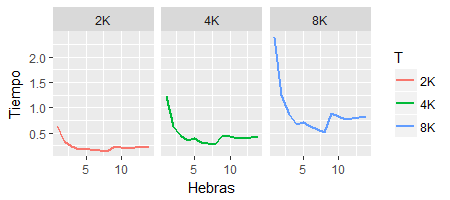
\includegraphics[width=\columnwidth]{tiempo-128px.png}
	\caption{Tiempo ejecución para T = \{2000, 4000, 8000\}}
	\label{fig:Figure1}
\end{figure}

\subsubsection{N = 256}
Aumentando el tamaño de grilla, se descubre lo siguiente:

\begin{figure}[h]
	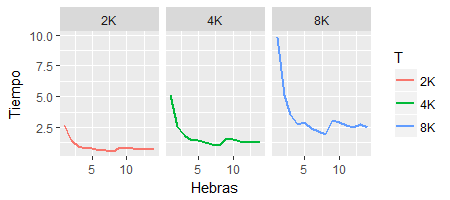
\includegraphics[width=\columnwidth]{tiempo-256px.png}
	\caption{Tiempo ejecución para T = \{2000, 4000, 8000\}}
	\label{fig:Figure2}
\end{figure}

\subsection{Speedup}
La métrica utilizada para calcular el \textit{speedup} será el relativo, el cual se expresa de la siguiente forma:

\[
	S_{relativo}(I, H) = \frac{tiempo\, resolv.\, I\, usando\, programa\, Q\, y\, 1\, hebra}{tiempo\, resolv.\, I\, usando\, programa\, Q\, y\, H\, hebras}
\]

\subsubsection{N = 128}
El resultado del análisis de rendimiento arroja lo siguiente:

\begin{figure}[h]
	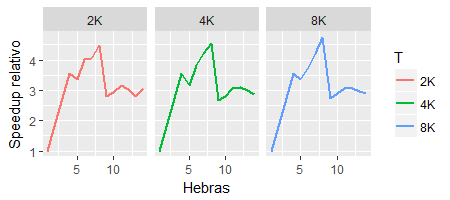
\includegraphics[width=\columnwidth]{srel-128px.png}
	\caption{Speedup relativo para T = \{2000, 4000, 8000\}}
	\label{fig:Figure3}
\end{figure}

\subsubsection{N = 256}
Mismo análisis con tamaño de grilla incrementado produce:

\begin{figure}[h]
	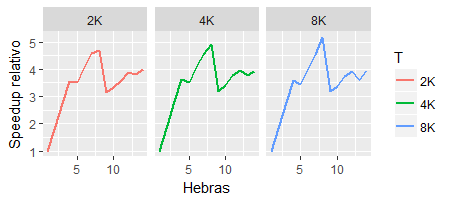
\includegraphics[width=\columnwidth]{srel-256px.png}
	\caption{Speedup relativo para T = \{2000, 4000, 8000\}}
	\label{fig:Figure4}
\end{figure}

\FloatBarrier

\subsection{Eficiencia}
La eficiencia fue calculada por medio la siguiente ecuación:

\[
	E(H) = \frac{S_{relativo}(I, 1)}{S_{relativo}(I, H) * H}
\]

Los resultados arrojados por el cálculo de la eficiencia son los siguientes:

\subsubsection{N = 128}
Mismo análisis con tamaño de grilla incrementado produce:

\begin{figure}[h]
	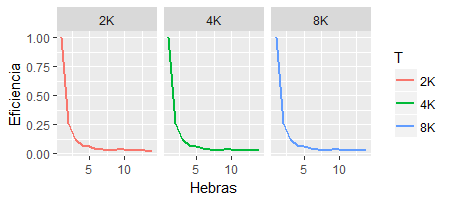
\includegraphics[width=\columnwidth]{efic-128px.png}
	\caption{Speedup relativo para T = \{2000, 4000, 8000\}}
	\label{fig:Figure5}
\end{figure}

\subsubsection{N = 256}
Mismo análisis con tamaño de grilla incrementado produce:

\begin{figure}[h]
	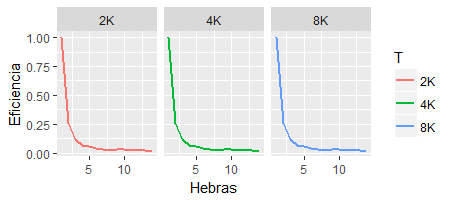
\includegraphics[width=\columnwidth]{efic-256px.png}
	\caption{Speedup relativo para T = \{2000, 4000, 8000\}}
	\label{fig:Figure6}
\end{figure}

\end{document}
